% !TeX spellcheck = en_US
% !TeX root = notes.tex
\subsection{Wireless}
\begin{figure}[H]
	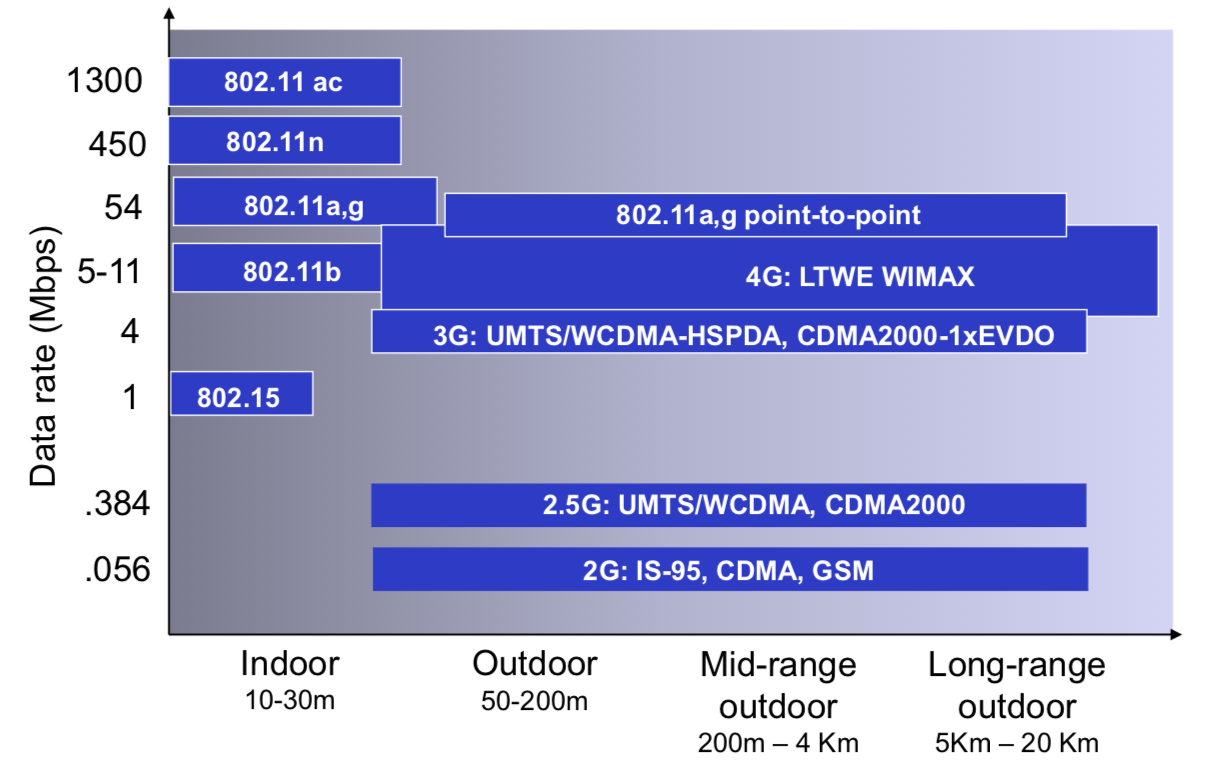
\includegraphics[width=\linewidth]{wifi}
	\centering
	\caption{Characteristics of selected wireless links}
\end{figure}
\subsubsection{Infrastructure mode}
\begin{itemize}
	\item base station connects mobiles into wired network
	\item handoff: mobile changes base station providing connection into wired network
\end{itemize}
\subsubsection{Ad Hoc mode}
\begin{itemize}
	\item no base stations
	\item nodes can only transmit to other nodes within link coverage
	\item nodes organize themselves into a network: route among themselves
\end{itemize}
\begin{table}[H]
	\centering
	\caption{Wireless Network Taxonomy}
	\begin{tabular}{p{2.5cm}|p{3cm}p{3cm}}
		\toprule
		&\textbf{single hop} & \textbf{multiple hops}\\
		\midrule
		\textbf{infrastructure (e.g. APs)} & host connects to base station (WiFi, WiMAX, cellular) which connects to larger Internet & host may have to relay through several wireless nodes to connect to larger Internet: mesh net\\
		\midrule
		\textbf{no infrastructure} & no base station, no connection to larger Internet (Bluetooth, ad hoc nets) & no base station, no connection to larger Internet. May have to relay to reach another given wireless node. MANET, VANET\\
		\bottomrule
	\end{tabular}
\end{table}
\subsubsection{Wireless Link Characteristics}
\textbf{important} difference from wired link...
\begin{description}
	\item[decreased signal strength:] radio signal attenuates as it propagates through matter (path loss)
	\item[interference from other sources:] standardized wireless network frequencies (e.g. 2.4GHz) shared by other devices (e.g. phone); devices (motors) interfere as well
	\item[multipath propagation:] radio signal reflects off objects ground, arriving ad destination at slightly different times
\end{description}
...make communication across (even a point to point) wireless link much more ``difficult''\\
SNR: signal-to-noise ratio. Larger SNR -- easier to extract signal from noise (a ``good thing'')\\
\textbf{SNR versus BER tradeoffs}
\begin{description}
	\item[given physical layer:] increase power $\rightarrow$ increase SNR $\rightarrow$ decrease BER
	\item[given SNR:] choose physical layer that meets BER requirement, giving highest throughput (SNR may change with mobility: dynamically adapt physical layer (modulation technique, rate)
\end{description}
\subsubsection{Code Division Multiple Access (CDMA)}
\begin{itemize}
	\item unique ``code'' assigned to each user; i.e. code set partitioning
	\begin{itemize}
		\item all users share same frequency, but each user has own ``chipping'' sequence (i.e. code) to encode data
		\item allows multiple users to ``coexist'' and transmit simultaneously with minimal interference (if codes are ``orthogonal'')
	\end{itemize}
	\item \textbf{encoded signal} = (original data) $\times$ (chipping sequence)
	\item \textbf{decoding:} inner-product of encoded signal and chipping sequence
\end{itemize}

\subsection{IEEE 802.11 Wireless LAN}
\textbf{802.11b}
\begin{itemize}
	\item 2.4 - 5 GHz unlicensed spectrum
	\item up to 11 Mbps
	\item direct sequence spread spectrum (DSSS) in physical layer (all hosts use same chipping code)
\end{itemize}
\textbf{802.11a}
\begin{itemize}
	\item 5 - 6 GHz range
	\item up to 54 Mbps
\end{itemize}
\textbf{802.11g}
\begin{itemize}
	\item 2.4 - 5 GHz
	\item up to 54 Mbps
\end{itemize}
\textbf{802.11n:} multiple antennae
\begin{itemize}
	\item 2.4 - 5 GHz range
	\item up to 200 Mbps
\end{itemize}
All use CSMA/CA for multiple access. All have base-station and ad-hoc network versions
\subsubsection{802.11 LAN architecture}
\begin{itemize}
	\item wireless host communicates with base station (base station = access point (AP))
	\item \textbf{Basic Service Set (BSS)} (aka ``cell'') in infrastructure mode contains:
	\begin{itemize}
		\item wireless hosts
		\item access point (AP): base station
		\item ad hoc mode: hosts only
	\end{itemize}
\end{itemize}
\subsubsection{Channels, association}
\begin{itemize}
	\item 802.11b: 2.4GHz - 2.485GHz spectrum divided into 11 channels at different frequencies
	\begin{itemize}
		\item AP admin chooses frequency for AP
		\item interference possible: channel can be same as that chosen by neighboring AP
	\end{itemize}
	\item host: must \textbf{associate} with an AP
	\begin{itemize}
		\item scans channels, listening for \textit{beacon frames} containing AP's name (SSID) and MAC address
		\item selects AP to associate with
		\item may perform authentication
		\item will typically run DHCP to get IP address in AP's subnet
	\end{itemize}
\end{itemize}
\begin{leftbar}
	802.11 has no collision detection
\end{leftbar}
\subsubsection{IEEE 802.11 MAC Protocol: CSMA/CA}
\textbf{802.11 sender}
\begin{enumerate}
	\item if sense channel idle for \textbf{DIFS} then transmit entire frame (no CD)
	\item if sense channel busy then:
	\begin{enumerate}
		\item start random backoff time
		\item timer counts down while channel idle
		\item transmit when timer expires
		\item if no ACK, increase random backoff interval, repeat 2
	\end{enumerate}
\end{enumerate}
\textbf{802.11 receiver}
If frame received OK $\rightarrow$ return ACK after \textbf{SIFS} (ACK needed due to hidden terminal problem)
\begin{figure}[H]
	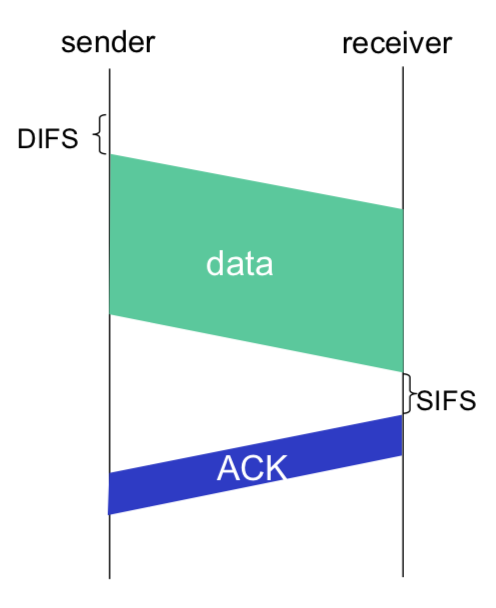
\includegraphics[width=0.5\linewidth]{proto}
	\centering
	\caption{802.11 CSMA/CA}
\end{figure}
\textbf{Avoiding Collisions}
\begin{itemize}
	\item sender first transmits \textit{small} request-to-send (RTS) packets to BS using CSMA (RTSs may still collide with each other (but they're short)
	\item BS broadcasts clear-to-send (CTS) in response to RTS
	\item CTS heard by all nodes (sender transmits data frame, other stations defer transmissions
\end{itemize}
\end{multicols*}
\subsubsection{802.11 frame: addressing}
\begin{table}[H]
	\centering
	\caption{802.11 frame}
	\begin{tabular}{cccccp{1.8cm}ccc}
		2&2&6&6&6&2&6&0-2312&4\\
		\midrule
		frame control & duration & address 1 & address 2 & address 3 & sequence control & address 4 & payload & CRC
	\end{tabular}
\end{table}
\begin{table}[H]
	\centering
	\caption{Frame Control Break Down}
	\begin{tabular}{p{1.5cm}cccp{0.8cm}cccccc}
		2&2&4&1&1&1&1&1&1&1&1\\
		\midrule
		Protocol version & Type & Subtype & To AP & From AP & More frag & Retry & Power mgt & More data & WEP & Rsvd
	\end{tabular}
\end{table}
\begin{multicols*}{2}
\begin{description}
	\item[Address 1:] MAC address of wireless host or AP to receive this frame
	\item[Address 2:] MAC address of wireless host or AP transmitting this frame
	\item[Address 3:] MAC address of router interface to which AP is attached
	\item[Address 4:] used only in ad hoc mode
\end{description}
\subsection{802.11 Power Management}
\begin{itemize}
	\item node-to-AP: Sleeping till next frame (AP knows not to transmit frames to this node, node wakes up before next beacon frame)
	\item beacon frame: contains list of mobiles with AP-to-mobile frames waiting to be sent (node will stay awake if AP-to-mobile frames to be sent; otherwise sleep again until next beacon frame
\end{itemize}
\subsection{802.15: Personal Area Network}
\begin{itemize}
	\item less than 10m diameter
	\item replacement for cables (mouse, keyboard, headphones)
	\item ad hoc: no infrastructure
	\item master/slaves: (slaves request permission to send (to master), master grants requests)
	\item 802.15: evolved from Bluetooth specification (2.4 - 2.5 GHz radio band, up to 721 kbps)
\end{itemize}
\begin{figure}[H]
	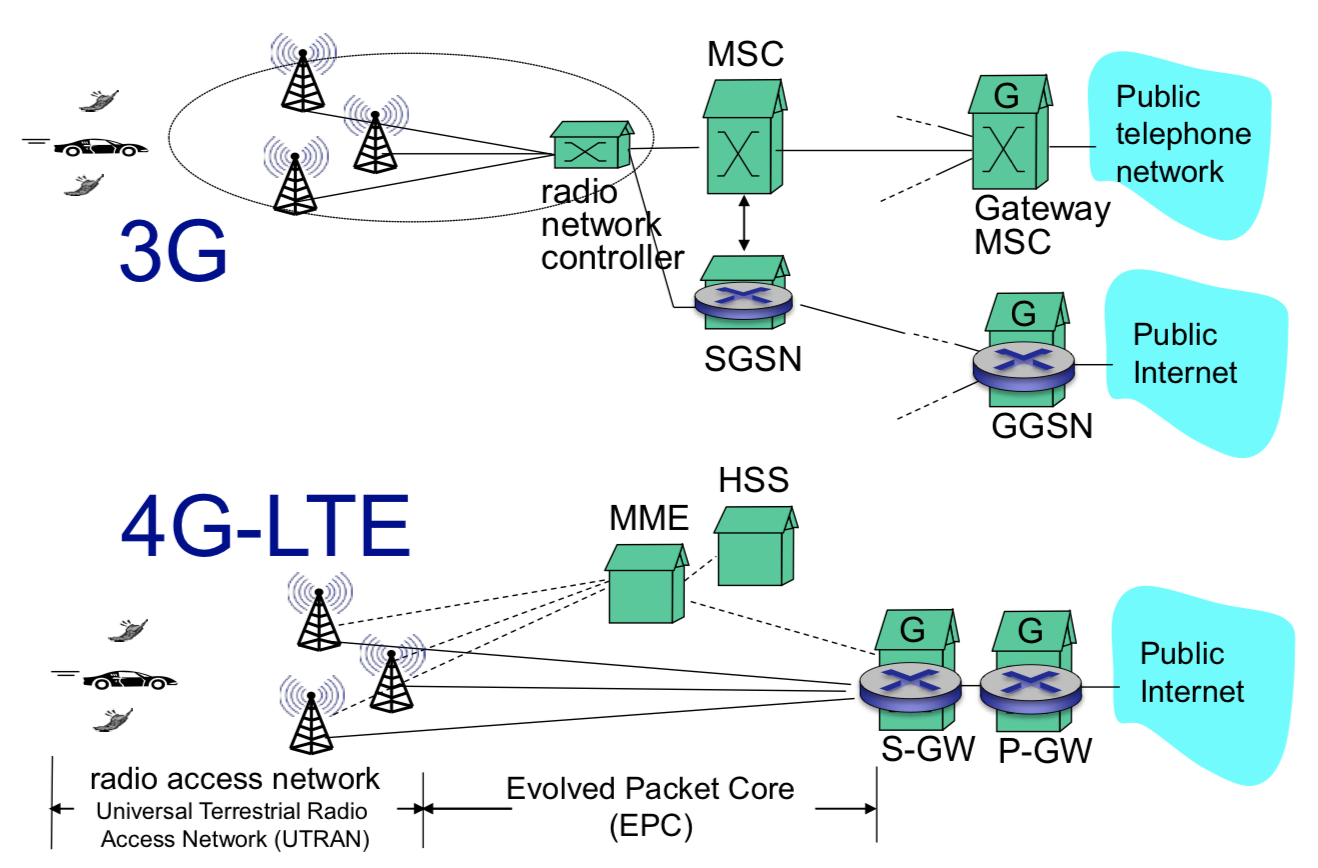
\includegraphics[width=\linewidth]{4G}
	\centering
	\caption{3G vs 4G LTE}
\end{figure}